\documentclass[pdftex,cig,slideColor]{pp4slides}
\usepackage{amsmath}
\usepackage{mpmulti}
\usepackage{multirow}
\usepackage{amsfonts}
\usepackage{pifont}
\usepackage{rotating} % use turn environment

\title{PyLith}
\subtitle{}
\author{Brad Aagaard, Charles Williams, Matthew Knepley, \\[10pt]
  Sue Kientz and Leif Strand}
\institution{
\includegraphics[height=2cm]{../logos/cig}}
\date{June 22, 2009}

% --------------------------------------------------------- DOCUMENT
\begin{document}

% ------------------------------------------------------------ SLIDE
\maketitle
\vfill

% ------------------------------------------------------------ SLIDE
\foilhead{PyLith}
  \summary{What is it good for?}

  \begin{itemize}
  \item Elasticity problems where geometry does not change significantly
  \item Quasi-static crustal deformation
    \begin{itemize}
    \item Strain accumulation associated with interseismic deformation
    \item Post-seismic relaxation of the crust
    \item Volcanic deformation associated with magma chambers and/or dikes
    \end{itemize}
  \item Dynamic rupture and wave propagation
    \begin{itemize}
    \item Kinematic (prescribed) earthquake ruptures
    \item Local/regional ground-motion modeling
    \end{itemize}
  \end{itemize}

\bgadd{\vspace*{7.9in}%
  \begin{center}%
    
\includegraphics[height=14mm]{../logos/cig}
  \end{center}}

% ------------------------------------------------------------ SLIDE
\foilhead{Crustal Deformation Modeling}
  \summary{Overview of workflow for typical research problem}

  \vfill
  \begin{center}
    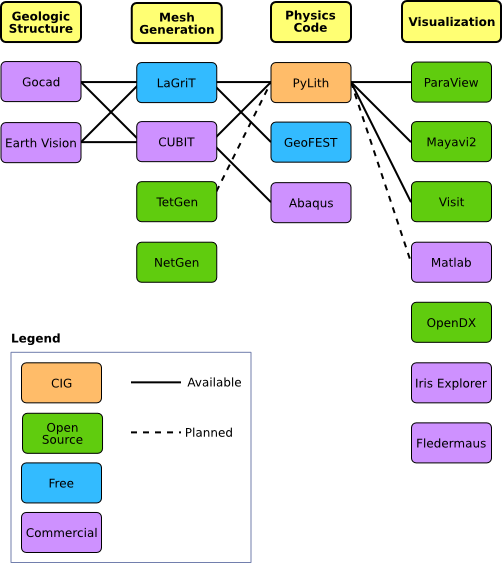
\includegraphics[scale=0.9]{figs/workflow}
  \end{center}

% ------------------------------------------------------------ SLIDE
\foilhead{Features in PyLith 1.4}
  \summary{}

  \begin{itemize}
  \item Time integration schemes
    \begin{itemize}
    \item Implicit time stepping for quasi-static problems
    \item Explicit time stepping for dynamic problems
    \end{itemize}
  \item Bulk constitutive models
    \begin{itemize}
    \item Elastic model (1-D, 2-D, and 3-D)
    \item Linear and Generalized Maxwell viscoelastic models (3-D)
    \item Power-law viscoelastic model (3-D)
    \end{itemize}
  \item Boundary and interface conditions
    \begin{itemize}
    \item Time-dependent Dirichlet boundary conditions
    \item Time-dependent Neumann (traction) boundary conditions
    \item Absorbing boundary conditions
    \item Kinematic (prescribed slip) fault interfaces w/multiple ruptures
    \item Time-dependent point forces
    \item Gravitational body forces
    \end{itemize}
  \end{itemize}

% ------------------------------------------------------------ SLIDE
\foilhead{Features in PyLith 1.4 (cont.)}
  \summary{}

  \begin{itemize}
  \item Automatic and user-controlled time stepping
  \item Ability to specify initial stress state
  \item Importing meshes
    \begin{itemize}
    \item LaGriT: GMV/Pset
    \item CUBIT: Exodus II
    \item ASCII: PyLith mesh ASCII format (intended for toy problems only)
    \end{itemize}
  \item Output: VTK files
    \begin{itemize}
    \item Solution over volume
    \item Solution over surface boundary
    \item State variables (e.g., stress and strain) for each material
    \item Fault information (e.g., slip and tractions)
    \end{itemize}
  \item Automatic conversion of units for all parameters
  \end{itemize}

% ------------------------------------------------------------ SLIDE
\foilhead{PyLith 1.4 Performance}
  \summary{PyLith 1.4 is $\sim$5\% faster and uses $\sim$50\% less memory than PyLith 1.3}

  \vfill
  \begin{center}
    \includegraphics[scale=1.0]{figs/benchmark_scaling}
  \end{center}
  \vfill

% ------------------------------------------------------------ SLIDE
\foilhead{PyLith 1.x: Planned Releases}
  \summary{Current productivity is about 2 feature releases per year}

  \begin{itemize}
  \item PyLith 1.5: anticipate release in late 2009 or early 2010
    \begin{itemize}
    \item Fault constitutive behavior with several widely used friction models
    \item Ability to specify initial strain and state variables
    \end{itemize}
  \item PyLith 1.6: Large deformations and finite strain
  \item PyLith 1.7: Automation of 4-D Green's functions
  \item PyLith 1.8: Coupling of quasi-static and dynamic simulations
  \end{itemize}
  
% ------------------------------------------------------------ SLIDE
\foilhead{PyLith Design Objective}
  \summary{Want a code developed for and by the community}
  
  \begin{itemize}
  \item Modular
    \begin{itemize}
    \item Users can swap modules to run the problem of interest
    \end{itemize}
  \item Scalable
    \begin{itemize}
    \item Code runs on one to a thousand processors efficiently
    \end{itemize}    
  \item Extensible
    \begin{itemize}
    \item Expert users can add functionality to solve their problem
      without polluting main code
    \end{itemize}
  \end{itemize}

% ------------------------------------------------------------ SLIDE
\foilhead{PyLith is a Community Code}
  \summary{Success of code depends on community participation}

  \begin{itemize}
  \item End-users (anyone who uses the code)
    \begin{itemize}
    \item Help define and prioritize features that should be added
    \item Report bugs/problems and suggest improvements
    \end{itemize}
  \item Expert users
    \begin{itemize}
    \item Help test alpha versions of releases
    \item Run benchmarks and report results
    \item Contribute meshing and visualization examples to documentation
    \item Add features following template (e.g., constitutive models)
    \end{itemize}
  \item Developer
    \begin{itemize}
    \item Define development strategy 
    \item Implement new features and tests
    \item Write documentation
    \end{itemize}
  \end{itemize}

% ------------------------------------------------------------ SLIDE
\foilhead{PyLith Design: Focus on Geodynamics}
  \summary{Leverage packages developed by computational scientists}

  \vfill
  \begin{center}
    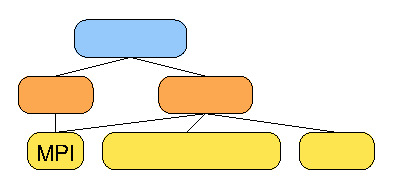
\includegraphics[scale=0.9]{figs/packages}
  \end{center}

% ------------------------------------------------------------ SLIDE
\foilhead{PyLith Design: Code Architecture}
  \summary{Flexible and modular with good performance}

  \begin{itemize}
  \item Top-level code written in Python
    \begin{itemize}
    \item Expressive, high-level, object-oriented language
    \item Dynamic typing allows adding additional modules at runtime
    \item Convenient scripting
    \end{itemize}
  \item Low-level code written in C++
    \begin{itemize}
    \item Compiled (fast execution), object oriented language
    \end{itemize}
  \item Bindings to glue Python \& C++ together
    \begin{itemize}
    \item SWIG generates code for calling C++ functions from Python
    \end{itemize}
  \end{itemize}

% ------------------------------------------------------------ SLIDE
\foilhead{PyLith Design}
 \summary{Tests, tests, and more tests ($>$1100 in all)}
 
 \begin{itemize}
 \item Create tests for nearly every function during development
   \begin{itemize}
   \item Remove most bugs during initial implementation
   \item Isolate and expose bugs at origin
   \end{itemize}
 \item Create new tests to expose bugs reported
   \begin{itemize}
   \item Prevent bugs from reoccurring
   \end{itemize}
 \item Rerun tests whenever code is changed
   \begin{itemize}
   \item Allows optimization of performance with quality control
   \item Code continually improves
   \end{itemize}
 \end{itemize}
  
% ------------------------------------------------------------ SLIDE
\foilhead{Example of Automated Building and Testing}
  \summary{Test written to expose bug, buildbot shows tests fail}

 \begin{center}
   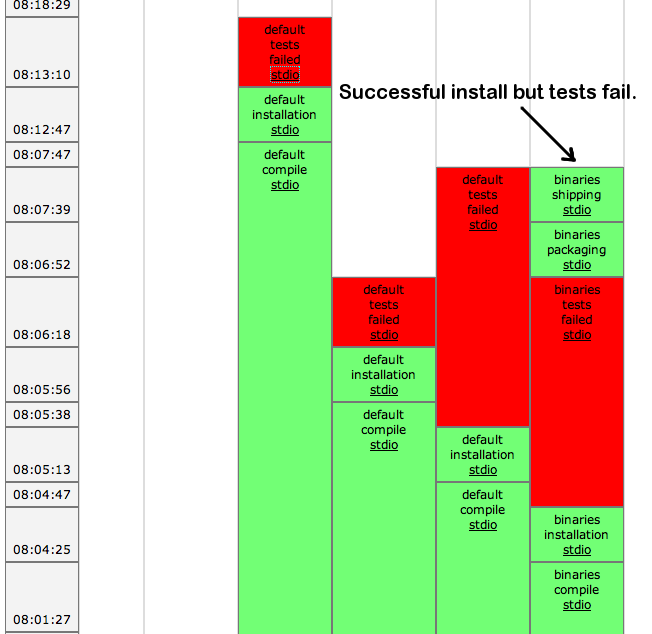
\includegraphics[scale=0.68]{figs/buildbotfail}
 \end{center}
  
% ------------------------------------------------------------ SLIDE
\foilhead{Automated Building and Testing}
 \summary{Bug is fixed, buildbot shows tests pass}

 \begin{center}
   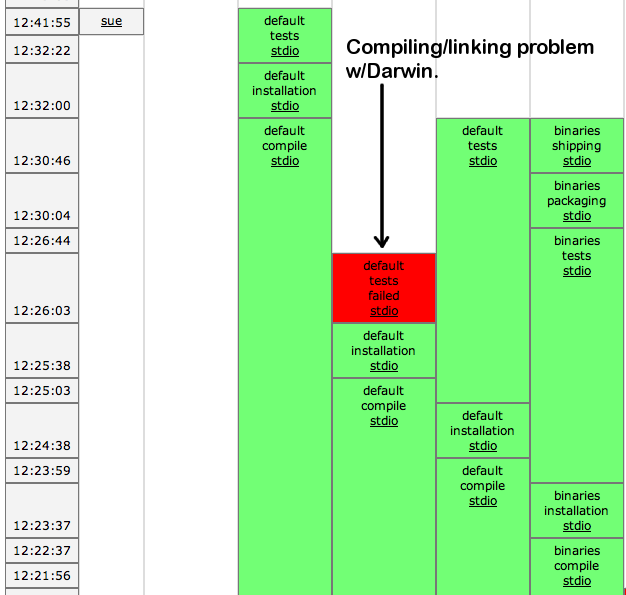
\includegraphics[scale=0.68]{figs/buildbotsuccess}
 \end{center}
  
% ------------------------------------------------------------ SLIDE
\foilhead{Implementation: Finite-Element Data Structures}
 \summary{Use Sieve for storage and manipulating mesh information}
 
 \begin{itemize}
 \item PyLith makes only a few MPI calls
 \item Data structures are independent of basis functions and
   reference cells
   \begin{itemize}
   \item Same code for many cell shapes and types
   \item Physics implementation limits code, not data structures
   \end{itemize}
 \item Sieve routines force adhering to finite-element formulation
   \begin{itemize}
   \item Do not have access to underlying storage
   \item Manipulations must be done using Sieve interface
   \item Only valid finite-element manipulation is allowed
   \end{itemize}
 \end{itemize}
  
% ------------------------------------------------------------ SLIDE
\foilhead{Implementation: Fault Interfaces}
 \summary{Use cohesive cells to control fault behavior}
 
  \vfill
  \begin{center}
    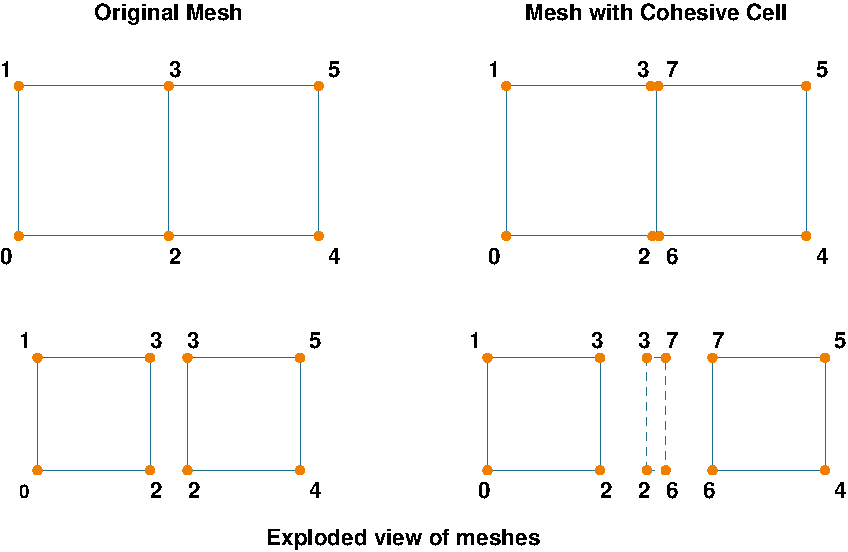
\includegraphics[scale=1.5]{figs/quad4cohesive}
  \end{center}

% ------------------------------------------------------------ SLIDE
\foilhead{Kinematic (prescribed) slip earthquake ruptures}
  \summary{Use Lagrange multipliers to specify slip}

  \begin{itemize}
  \item System without cohesive cells
    \begin{equation}
      \underbar{A} \vec{u} = \vec{b} \nonumber
    \end{equation}
  \item System with cohesive cells
    \begin{equation}
      \left( \begin{array}{cc}
          \underbar{A} & \underbar{C}^T\\
          \underbar{C} & 0
        \end{array} \right)
      \left( \begin{array}{c}
          \vec{u}\\
          \vec{L}
        \end{array}\right)
      =
      \left( \begin{array}{c}
          \vec{b}\\
          \vec{D}
        \end{array} \right)
      \nonumber
    \end{equation}
  \end{itemize}
  
% ------------------------------------------------------------ SLIDE
\foilhead{Implementing Fault Slip with Lagrange multipliers}
 
 \begin{itemize}
 \item Advantages
   \begin{itemize}
   \item Fault implementation is local to cohesive cell
   \item Solution includes forces generating slip (Lagrange multipliers)
   \item Retains block structure of matrix (same number of DOF per vertex)
   \item Offsets in mesh mimic slip on natural faults
   \end{itemize}
 \item Disadvantages 
   \begin{itemize}
   \item Creates a saddle point problem (slower convergence)
   \item Mixes displacements and forces in solution
   \end{itemize}
 \end{itemize}
  
% ------------------------------------------------------------ SLIDE
%\foilhead{Benchmarking PyLith}
%  \summary{Savage and Prescott (1978): Repeated Strike-slip ruptures}
%
%  \movie{0.58in}{0.0in}{7.84in}{5.84in}{movies/savageprescott_domain}
 
% ------------------------------------------------------------ SLIDE
%\foilhead{Benchmarking PyLith}
%  \summary{Savage and Prescott (1978): Repeated Strike-slip ruptures}
%
%  \movie{0.58in}{0.0in}{7.84in}{5.84in}{movies/savageprescott_groundsurf}
 
% ------------------------------------------------------------ SLIDE
\foilhead{Benchmarking PyLith}
  \summary{Analytical solution from Savage and Prescott (1978)}

  \begin{itemize}
  \item Repeated rupture on a vertical, strike-slip fault
  \item Elastic layer over a linear Maxwell viscoelastic half-space
  \item Steady creep over bottom half of the elastic layer
  \end{itemize}
  
  \vfill
  \begin{center}
    \includegraphics[scale=0.8]{figs/savageprescott_soln}
  \end{center}
  
% ------------------------------------------------------------ SLIDE
\foilhead{Benchmarking PyLith}
  \summary{Simulation closely matches analytical solution during 10th eq cycle}

  \vfill
  \begin{center}
    \includegraphics[scale=1.2]{figs/savageprescott_profile9}
  \end{center}
  
% --------------------------------------------------------- DOCUMENT
\end{document}


% End of file
